% This is samplepaper.tex, a sample chapter demonstrating the
% LLNCS macro package for Springer Computer Science proceedings;
% Version 2.20 of 2017/10/04
%
\documentclass[runningheads]{llncs}
%
\usepackage{graphicx}
\usepackage{listings}
\usepackage{color}
\lstset{language=C++,
                basicstyle=\ttfamily,
                keywordstyle=\color{blue}\ttfamily,
                stringstyle=\color{red}\ttfamily,
                commentstyle=\color{green}\ttfamily,
                morecomment=[l][\color{magenta}]{#}
}
% Used for displaying a sample figure. If possible, figure files should
% be included in EPS format.
%
% If you use the hyperref package, please uncomment the following line
% to display URLs in blue roman font according to Springer's eBook style:
% \renewcommand\UrlFont{\color{blue}\rmfamily}

\begin{document}
%
\title{Raport tehnic asupra aplicatiei Mersul Trenurilor}
%
%\titlerunning{Abbreviated paper title}
% If the paper title is too long for the running head, you can set
% an abbreviated paper title here
%
\author{Andrei Moldoveanu, 2A2}
%
% First names are abbreviated in the running head.
% If there are more than two authors, 'et al.' is used.
%
\institute{Universitatea Alexandru Ioan Cuza, Facultatea de Informatica \\
\email{andrei.moldoveanu@info.uaic.ro}\\
\url{http://info.uaic.ro}}
%
\maketitle              % typeset the header of the contribution
%
\begin{abstract}
 In acest articol este descrisa o modalitate de implementare a unei aplicatii ce ofera utilizatorilor date despre mersul trenurilor, folosind ca protocol de comunicare UDP si metode de procesare a informatiilor concurente astfel incat se reduc cat mai mult timpii de raspuns al acesteia.

\keywords{Command design pattern  \and command queue \and threads \and \\ sockets.}
\end{abstract}
%
%
\section{Introducere}
\subsection{Motivatie}

 Mobilitatea reprezinta un aspect important in viata fiecarei persoane, iar trenurile sunt unele din cele mai importante mijloace de transport. In acest moment timpul este una dintre resursele cele mai de pret, astfel ca nu ne permitem sa il irosim. Nevoie de a avea date actualizate in timp real despre mersul trenurilor, informatii despre posibile abateri de la programul normal, cat si posibilitatea de a afla exact oferta de mobilitate pentru o anumita ruta, reprezinta motivatia care a stat la baza acestui articol. De asemenea un aspect important este lipsa unei aplicatii pentru trenuri in care utilizatorii sa fie implicati direct prin semnalarea posibilelor abateri de la orar.

\subsection{Scop}

 Mersul trenurilor reprezinta un pilon important in mobilitatea populatiei in fiecare zi, iar realizarea unei aplicatii care sa raspunda exact cerintelor utilizatorilor in cautare de informatii corecte, rapide si de actualitate reprezinta principalul scop al acestui articol.
\clearpage

\section{Tehnologii utilizate}

\indent Protocolul de comunicatie utilizat la nivelul transport este UDP. Acesta este un mod de comunicatie fara conexiune, spre deosebire de protocolul TCP, fapt ce conduce la pierderea informatiilor in timpul transferului. Mesajele circula de la un punct la altul al retelei fara sa se asigure ca cel care le primeste este disponibil si gata sa accepte datele. Pentru a suprima acest incovenient au fost introduse mechanisme care sa se asigure ca mesajele au ajuns la destinatar, cum ar fi trimiterea unui mesaj de la server catre client care sa confirme primirea mesajului, iar clientul in cazul in care nu primeste acest mesaj va retrimite pachetele de date. De asemenea fiecare pachet de date trimis este insotit de catre un id unic si o schema de numarare, iar atat serverul cat si clientul este responsabil de ignorarea duplicatelor in cazul in care acestea vor aparea, pentru reordonarea mesajelor, cat si de depistarea datagramelor lipsa. \\
\indent Scenariile de utilizare ale aplicatiei Mersul Trenurilor implica faptul ca este utilizata de multi utilizatori concomitent iar viteza de raspuns este un factor import, astfel ca protocolul UDP primeaza avand o viteza mai mare cauzata de putinele suprasarcini.\\
\indent Protocolul UDP reprezinta un mare avantaj in momentul in care ne confruntam cu o multitudine de mesaje ce trebuie procesate, deoarece ignorarea mesajelor devine o varianta viabila in momentul in care cozile pregatite pentru stocarea acestora devin pline. Aceste mesaje vor fi retrimise de catre clienti. Alternativa la TCP pentru aceste incidente ar presupune intreruperea conexiunilor. Acest avantaj cat si faptul ca implementarea unui protocol UDP este facila, a dus la alegerea acestui protocol pentru aplicatia Mersul Trenurilor.


\clearpage

\section{Arhitectura aplicatiei}

%diagrama arhitectura module
\begin{figure}[htp]
    \centering
    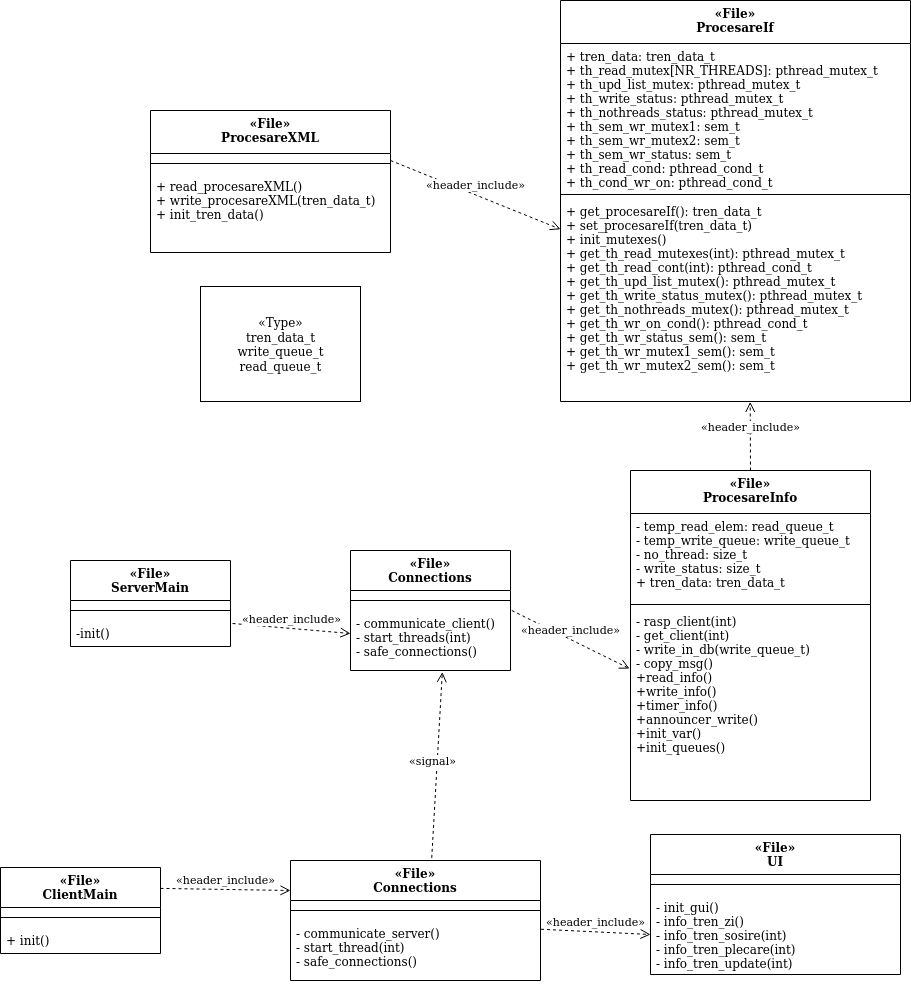
\includegraphics[width=13cm,height=13cm]{ms_file_diag.png}
    \caption{Diagrama arhitectura module}
\end{figure}

Aceasta aplicatie este compusa din doua componente, client si server. Implementarea ei este pe o retea de calculatoare care conecteaza cele doua componente. Partea de server din arhitectura contine functionalitatile principale, cum ar fi faptul ca oricati clienti se pot conecta la server si pot face request la anumite task-uri. Aceste task-uri vor fi procesate concurential, iar, in cazul in care va fi nevoie, rezultatul lor va fi transmis inapoi clientilor. Partea de client va pune la dispozitie utilizatorilor o interfata grafica prin itermediul careia acestia pot sa invoce cereri.

Modulele au fost impartite astfel incat sa nu existe dependente ciclice, iar diagrama de dependente a fost construita asemenea unui DAG (directed acyclic graph). De asemenea, modulele sunt dependente de cele mai stabile dintre acestea. Pentru a inversa dependenta probabila intre modulele \textit{ProcesareInfo} si \textit{ProcesareXMl} am introdus un nou modul cu rol de interfata \textit{ProcesareIf}. Aceasta dependeta era de evitat deoarece modulul \textit{ProcesareXML} este volatil si orice modificare in acest modul ar fi dus si la recompilarea si regandirea modulului \textit{ProcesareInfo}. Functiile din fiecare modul au fost alese astfel incat sa se schimbe pentru acelasi motiv si in acelasi timp, respectand astfel si principiul Common Closure.


%diagrama xml module
\begin{figure}[htp]
    \centering
    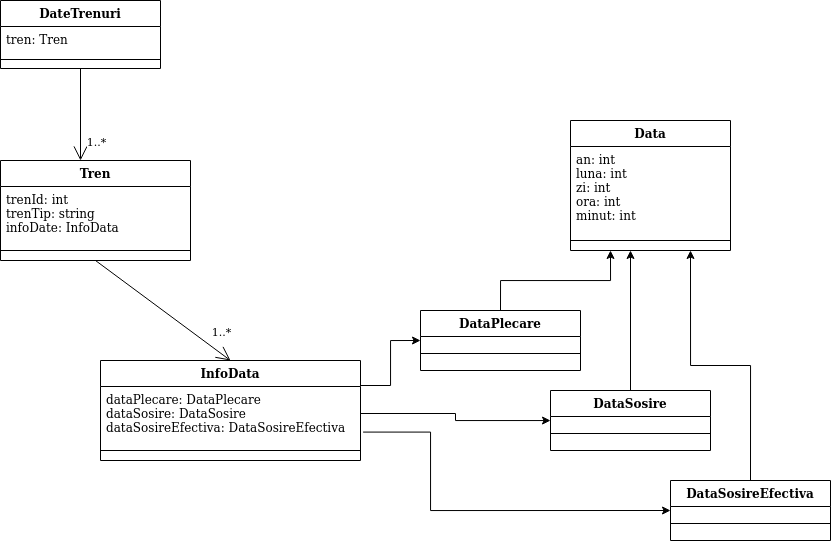
\includegraphics[width=13cm]{train_data_xml.png}
    \caption{Diagrama UML pentru schema XML}\label{fig2}
\end{figure}

In aceasta schema UML (figura~\ref{fig2}), sunt evidentiate proprietatile unui ansamblu ce poate sa contina unul sau mai multe trenuri. Fiecare tren contine un \textit{ID}, un \textit{tip} precum si \textit{InfoData}. \textit{InfoData} reprezinta intervalele orare la care un tren este asteptat sa plece sau sa ajunga intr-o statie, acestea avand acelasi tip de data si anume \textit{Data}. Concepte precum cardinalitate (un \textit{Tren} poate avea unul sau mai multe \textit{InfoData} sau \textit{DateTrenuri} contine unul sau mai multe \textit{trenuri}), mostenire (\textit{DataPlecare} mosteneste toate proprietatile unei \textit{Date}) sau relatii de dependenta (\textit{DateTrenuri} depinde de toate \textit{trenurile}) pot fi observate cu usurinta in aceasta diagrama.

%cod
\begin{lstlisting}[language=c++,caption={MersulTrenurilor.xml example}]
<dateTrenuri>
    <tren>
        <trenID>123</trenID>
        <trenTip>IR</trenTip>
        <infoData>
            <dataPlecare>
                <an>2021</an>
                <luna>01</luna>
                <zi>02</zi>
                <ora>14</ora>
                <minut>30</minut>
            </dataPlecare>
            <dataSosire>
                <an>2021</an>
                <luna>01</luna>
                <zi>02</zi>
                <ora>18</ora>
                <minut>00</minut>
            </dataSosire>
            <dataSosireEfectiva>
                <an>2021</an>
                <luna>01</luna>
                <zi>02</zi>
                <ora>18</ora>
                <minut>10</minut>
            </dataSosireEfectiva>
        </infoData>
        <infoData>
        ...
        </infoData>
    </tren>
    <tren>
    ...
    </tren>
</dateTrenuri>
\end{lstlisting}

\clearpage

\section{Detalii de implementare}
\subsection{Scenarii de utilizare}

%diagrama use case generala
\begin{figure}[htp]
    \centering
    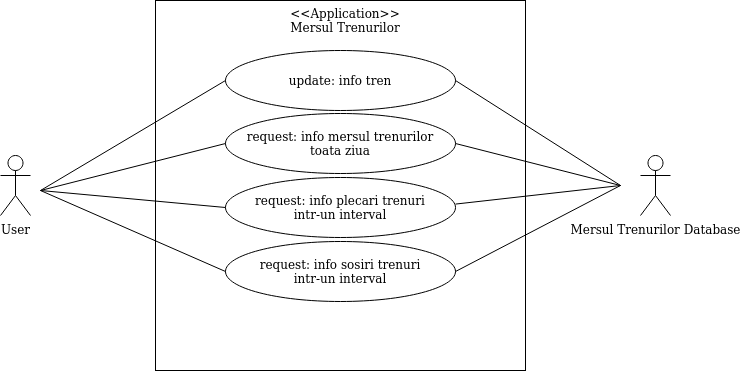
\includegraphics[width=12cm]{use-case1.png}
    \caption{Scenarii de utilizare aplicatie Mersul Trenurilor}
\end{figure}

\indent Prin intermediul aplicatiei Mersul Trenurilor utilizatorul poate avea acces in timp real la informatii referitoare la orarul trenurilor intr-un anumit interval, dar de asemenea poate updata informatii despre statusul unui anumit tren.

%diagrama use case generala
\begin{figure}[htp]
    \centering
    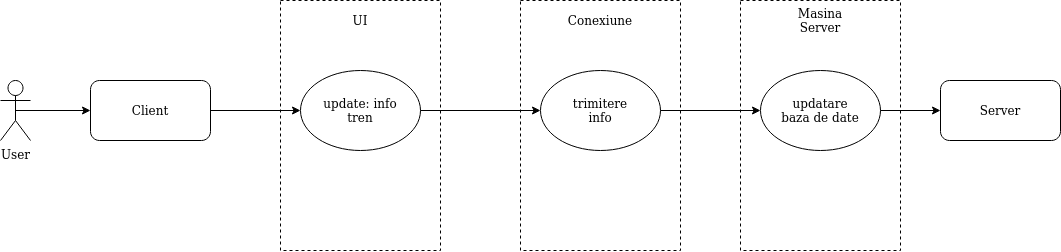
\includegraphics[width=14cm]{use_case_update.png}
    \caption{Scenarii de utilizare update}
\end{figure}
Din interfata grafica un user poate solicita updatarea starii unui tren identificat dupa un ID si un tip specificand abaterea acestuia, in unitati de timp, de la orarul normal. 
\clearpage

%diagrama use case generala
\begin{figure}[htp]
    \centering
    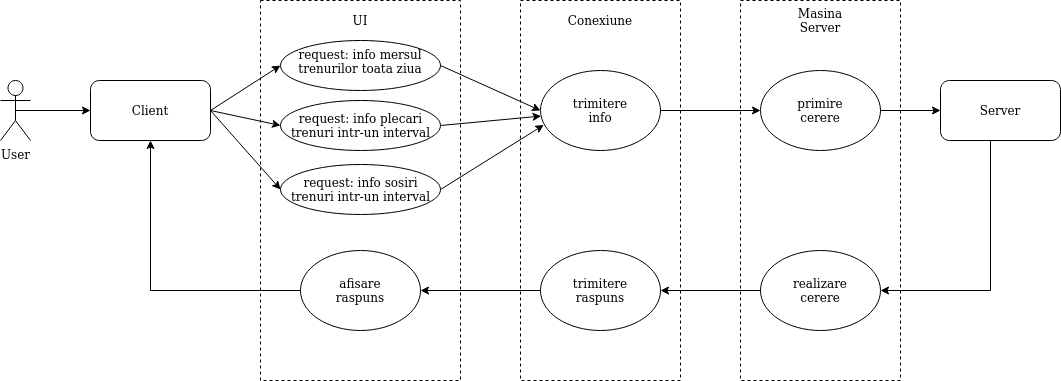
\includegraphics[width=14cm]{use_case_request.png}
    \caption{Scenarii de utilizare request}
\end{figure}

\indent Din interfata grafica un user poate solicita de la server informatii despre mersul trenurilor in ziua respectiva. Se mai pot solicita informatii despre plecari sau sosiri intr-un anumit interval orar. Aceste informatii vor fi furnizate conform cu planul, iar posibilile sosiri inainte sau dupa termenul original specificat in orar vor fi de asemenea transmise. Datele transmise vor fi afisate utilizatorului intr-o interfata grafica prietenoasa.

%cod
\indent Functiile au fost impartite astfel incat sa se respecte principiul SRP(Single Responsibility Principle) astfel ca fiecare sa aiba un singur motiv sa fie schimbat.

\begin{lstlisting} [language=c++,caption={sincronizare thread update cu thread-urile de request}]
while(1){
    sem_wait(get_th_wr_mutex2_sem());
    /* sinc cu thread-urile de request
     * semnalez ca vreau sa scriu */
    pthread_mutex_lock(get_th_write_status_mutex());
    write_status = 1;
    /* blochez thread-ul de request la sem */
    sem_wait(get_th_wr_status_sem_());

    /* astept semnalul ca toate thread-urile s-au oprit */
    /* verific daca nu cumva sunt toate oprite */
    pthread_mutex_lock(get_th_nothreads_mutex());
    if (no_threads != 0)
    {
      pthread_mutex_unlock(get_th_nothreads_mutex());
      pthread_cond_wait(get_th_wr_on_cond(), get_th_write_status_mutex());
    }
    else
      pthread_mutex_unlock(get_th_nothreads_mutex());

    /* transfer lista de update-uri */
    pthread_mutex_lock(get_th_upd_list_mutex());
    tmp_write_queue = (write_queue_t *)malloc(sizeof(write_queue_t));
    tmp_write_queue->primul = write_queue->primul;
    write_queue->primul = NULL;

    /* am terminat de transferat */
    pthread_mutex_unlock(get_th_upd_list_mutex());

    if (tmp_write_queue->primul != NULL)
    {
      write_in_db(tmp_write_queue);
    }
    else //ma intorc la semafor
    {
      free(tmp_write_queue);
      printf("nu am printat nimic in db\n\n");
    }
    /* semnalez thread-ul de request */
    write_status = 0; //modific statusul la write
    pthread_mutex_unlock(get_th_write_status_mutex());
    sem_post(get_th_wr_status_sem_());
    /* semnalez th ciclic */
    sem_post(get_th_wr_mutex1_sem());
}
\end{lstlisting}

Thread-ul pentru \textit{update}-uri are o bucla infinita in care se sincronizeaza cu thread-urile pentru partea de \textit{request}. \\ 
\indent In primul rand thread-ul de \textit{update} primeste ciclic un semnal de pornire de la un thread \textit{announcer} iar ca mecanism de sincronizare am folosit semafoare. Acest thread \textit{announcer} nu trimite semnal daca nu exista nici o modificare de facut. Thread-ul de update semnaleaza faptul ca vrea sa faca modificari in structura de date comuna modificand statusul de write, iar apoi asteapta ca toate thread-urile de \textit{request} sa se opreasca. In momentul in care ultimul thread de \textit{request} s-a oprit, el va primi signal sa continue recuperand lock-ul pus pe write (acest lock este important pentru ca thread-urile de \textit{request} pot sa fie suspendate deoarece nu au task-uri, iar daca sunt semnalate ca au primit task sa nu poate citi din structura de date). Astfel acesta transfera lista de modificari (in momentul transferarii se va sincroniza cu thread-ul care face citirile din socket). Se va continua cu scrierea in structura de date, iar dupa va fi modificat statusul de write, va fi eliberat lock-ul pus pe write si va fi incrementat semaforul care opreste toate thread-urile de request astfel incat acestea sa poate continua. Se va sincroniza de asemenea si thread-ul \textit{announcer}.


\clearpage
\begin{lstlisting} [language=c++,caption={sincronizare thread-uri de request cu thread-ul de update si cu thread-ul care asigneaza task-uri}]
static void get_client(int thread_id){
  while (read_queue_vec[thread_id]->urm->primul == NULL)
  {
    pthread_mutex_lock(get_th_nothreads_mutex());
    no_threads--;
    if (no_threads == 0)
    {
      /* semnal la thread-ul de update ca poate sa inceapa */
      pthread_cond_signal(get_th_wr_on_cond()); 
    }
    pthread_mutex_unlock(get_th_nothreads_mutex());
    pthread_cond_wait(get_th_read_cond(thread_id),
                    get_th_read_mutex(thread_id));
    pthread_mutex_lock(get_th_nothreads_mutex());
    no_threads++;
    pthread_mutex_unlock(get_th_nothreads_mutex());
  }
  /* vf daca se va scrie in database */
  pthread_mutex_lock(get_th_write_status_mutex());
  if (write_status == 1)
  { //write worker-ul a semnalat ca vrea sa scrie in database
    pthread_mutex_lock(get_th_nothreads_mutex());
    no_threads--;
    pthread_mutex_unlock(get_th_nothreads_mutex());
    if (no_threads == 0)
    {
      /* semnal la thread-ul de update ca poate sa inceapa */
      pthread_cond_signal(get_th_wr_on_cond()); 
    }
    pthread_mutex_unlock(get_th_write_status_mutex());
    sem_wait(get_th_wr_status_sem_());
    sem_post(get_th_wr_status_sem_());
    pthread_mutex_lock(get_th_nothreads_mutex());
    no_threads++;
    pthread_mutex_unlock(get_th_nothreads_mutex());
  }
  else //nu se scrie in database si pot continua
  {
    pthread_mutex_unlock(get_th_write_status_mutex());
  }
  copy_msg(); //copii mesajul din lista si il sterg
  pthread_mutex_unlock(get_th_read_mutex(thread_id));
}
\end{lstlisting}

Thread-urile de \textit{request} se vor sincroniza cu un thread worker de \textit{transfer} folosind mutex-uri iar daca nu au nimic de executat vor fi suspendate, decrementand numarul de thread-uri active. Sincronizarea cu thread-ul de \textit{update} este realizata prin mutex si semafoare astfel ca se va verifica de fiecare data statusul de write, iar daca acesta nu este setat pe 0 se va trece mai departe. Daca statusul de write este setat, atunci thread-urile de \textit{request} se vor bloca in semafor. Thread-urile de \textit{request} vor iesi pe rand din block-ul de pe semafor atunci cand thread-ul worker de \textit{update} il va incrementa (la sfarsitul modificarii structurii de date).

\section{Concluzii}

\indent Utilizarea protocolului UDP si sistemul de command queue implementat contribuie la o performanta buna a aplicatiei pe partea de procesare a cererilor si eliminare a blocajelor. \\
\indent Se pot extinde functionalitatile aplicatiei cu un mechanism de mediere a intarzierilor in momentul in care exista mai multe informatii despre acelasi tren. Acesta poate fi corelat cu un mecanism de ignorare selectiva a datagramelor in momentul in care stiva ce le stocheaza devine aproape plina. \\
\indent O alta directie de dezvoltare este de asemenea implementarea unui sistem astfel incat sa fie luata in considerarea si ruta dorita de catre utilizator. Aceasta functionalitate se poate extinde astfel incat sa fie returnat traseul in functie de durata, lungime sau alti parametri intr-o ordine apriori stabilita.


%
% ---- Bibliography ----
%
% BibTeX users should specify bibliography style 'splncs04'.
% References will then be sorted and formatted in the correct style.
%
% \bibliographystyle{splncs04}
% \bibliography{mybibliography}
%
\begin{thebibliography}{8}
\bibitem{ref_book1}
David R. Hanson: C Interfaces and Implementations. Addison-Wesley,
United States of America (1997)

\bibitem{ref_book2}
Robert C. Martin: Clean Architecture. Prentice Hall,
United States of America (2018)

\bibitem{ref_url1}
UML diagrams Homepage, \url{https://www.uml-diagrams.org}.


\bibitem{ref_url2}
IBM Homepage, \url{https://www.ibm.com}.

\bibitem{ref_url3}
Modeling C applications in UML with files and structures, \url{http://signal-processing.mil-embedded.com/articles/modeling-applications-uml-files-structures/}.

\bibitem{ref_url4}
POSIX Threads Programming, \url{https://computing.llnl.gov/tutorials/pthreads/}.

\bibitem{ref_url5}
man page, \url{https://linux.die.net/man/}.

\bibitem{ref_url6}
semaphores, \url{https://docs.oracle.com/cd/E19683-01/806-6867/6jfpgdcnj/index.html}

\bibitem{ref_url7}
Computer Networks, \url{https://profs.info.uaic.ro/~computernetworks/cursullaboratorul.php}

\bibitem{ref_article1}
K. Lano, S. Yassipour-Tehrani, H. Alfraihi: Transformation from UML to C: A large-scale example of MDD for model transformation development. Dept. of Informatics, King's College London, March 1, 2017


\end{thebibliography}
\end{document}

